\documentclass[10pt,a4paper]{article}
\usepackage[a4paper, left=3cm, right=3cm, top=3cm, bottom=3cm, headsep=10mm, footskip=12mm]{geometry}
\usepackage[T1]{fontenc}
\usepackage[ngerman, english]{babel}    % mehrsprachiger Textsatz
% babel: letzte Sprache in Optionen zeigt die Sprache des Dokumentes
% und kann durch den Befehl \selectlanguage{} geaendert werden
% Passen Sie die Optionen des babel-Paketes nach Bedarf an!
\usepackage{float}
\usepackage{graphicx}
\usepackage{url}
\usepackage{pdflscape}
\usepackage{mathtools}
\usepackage{amssymb, amsmath, amstext}
\usepackage{amsthm}
\usepackage{xcolor}
\usepackage{nameref}
\usepackage{siunitx}
\usepackage{makecell}
\usepackage{hyperref}
\usepackage{enumitem}
\usepackage[superscript,biblabel]{cite}
\usepackage{caption}
\usepackage{subcaption}
\usepackage{tabularx} 			% Tabellen erzeugen
\usepackage{multirow}			 % Zeilen in Tabellenbearbeitung
\usepackage{multicol} 			% Spalten in Tabellenbearbeitung 
\usepackage{lmodern}                        % Ersatz fuer Computer Modern-Schriften 
\usepackage{amsmath}                                           % zum besseren Aussehen am Bildschirm
\usepackage{booktabs} % für schönere Tabellen
\usepackage{sidecap}
\usepackage{rotating} % für die Landscape-Umgebung
\usepackage{afterpage}
\definecolor{Bluetitle}{HTML}{1F3864}
\definecolor{Greyish}{HTML}{5A5A5A}
\renewcommand{\refname}{Reference}
\usepackage{array,multirow}
\newcommand{\specialcell}[2][c]{%
	\begin{tabular}[#1]{@{}c@{}}#2\end{tabular}}




\begin{document}
	
	\begin{titlepage}
		\begin{center}
			\begin{figure}[h!tbp]
				
\includegraphics[width=\linewidth]{HUlogo.PNG}
			\end{figure}
			\vspace*{2 cm}
			
			\textcolor{Bluetitle}{\textbf{\huge Qualitative und quantitative Charakterisierung
					der Photosynthesepigmente}}\par
			
			\vspace*{2cm}
			
			\textcolor{Greyish}{\textbf{Versuchsdurchführende}}\par
			\textcolor{Greyish}{Oscar Moore (634083)}\par
			\textcolor{Greyish}{Frido (....)}\par
			\textcolor{Greyish}{Philipp.. (...)}\par
			\textcolor{Greyish}{Daniel... (...)}\par
			\textcolor{Greyish}{Huyen Anh Nguyen (572309)}\par
			\vspace*{0.5cm}
			\textcolor{Greyish}{\textbf{Versuchsort}}\par
			\textcolor{Greyish}{Campus Nord, Haus 9}\par
			\textcolor{Greyish}{R2002}\par
			\vspace*{0.5cm}
			\textcolor{Greyish}{\textbf{Versuchsbetreuer}}\par
			\textcolor{Greyish}{Prof. Dr. rer. nat. Bernhard Grimm}\par
			
			\vspace*{2 cm}
			
			\textcolor{Greyish}{11. Juni 2024}\par
			

			
			
		\end{center}
	\end{titlepage}
		
		\tableofcontents
		

	
	\newpage
	\section{Einführung}
	

	
	\section{Material und Methode}
	Für diesen Versuch wurde die Tabakpflanze Nicotiana tabacum als Wildtyp und die antisense FC1 mutierte Variante verwendet.\\
	Die Verdünnungen und Homogenisieren wurde jeweils auf Eis durchgeführt.
		\subsection{Herstellung des Pigmentextraktes}
		Es wurde 0.9965g Pflanzenmaterial des Wildtypens und 0.9960g des Mutantes eingewogen.\\
		Die Proben wurden mit kalten basischen Aceton (100$\%$ Aceton und 20 mM NH$_4$OH) homogenisiert und über einem Miraclothfilter in einem 50 mL Falconröhrchen filtriert. Homogenisierung mit Quarzsand wurde zwei Mal durchgeführt und das Homogenisat in einem 15 mL Falconröhrchen vereint.
		
		\subsection{Photometrische Bestimmung Chlorophylle a und b}
		Um eine quantitative Bestimmung von  Chlorophyll a und b durchzuführen, wurden zuerst 0.2ml  des Wildtyp-Extrakts (WT) und des der Mutante (MU) in ein 1,5ml Reaktionsgefäß überführt. Anschließend wurde ein Verhälltnis von 1:5 geschaffen, indem 0.8ml basisches Aceton hinzugegeben wurde.  \\
		Das Gemisch wurde gevortext und für eine Minute bei 15.000 rpm herunterzentrifugiert.
		Die photometrische Bestimmung von 1 mL Probevolumen erfolgte bei 470nm, 646nm, 663nm und 720nm wobei 720nm Wellenlänge als Maß für Verunreinigung diente und 470nm als nicht relevanter Kontrollwert.\\
		Als Blank-Lösung wurde das Extraktionslösung (basisches Aceton) verwendet.
		
		\subsection{DC-Trennung Chlorophylle und Carotinoide}
		5 mL des basischen Pigmentextraktes vom Wildtyp und Mutant wurde mit 1 mL Petrolether versetzt und 3 mal vorsichtig invertiert.
		Die Proben wurden für 10 Minuten im Eis inkubiert und die obere dunkelgrüne Phase für die weiteren Versuchen in einem 1.5 mL Eppendorf Tube überführt.\\
		\\
		50 Mikroliter von den beiden Proben wurden auf einer Dünnschichtchromatographie-Platte (abgekürzt: DC-Platte) als breite Bande aufgetragen.
		In einem mit Laufmittel (Petrolether/Aceton/Isopropanol/Wasser, 400:80:48:1)-abgesättigte DC-Kammer wird die DC-Platte inkubiert und der Lauf wurde gestoppt, als diese 5 mm Abstand zur DC-Plattenkante erreicht hatte.
		\subsection{Fluoreszenz des Chlorophyllextractes}
		\subsection{Phäophytinbildung}
	
	\section{Ergebnis}
		\subsection{Konzentrationsbestimmung von Chlorophylle im Rohextrakt}
		Die Konzentration von Chlorophyll a und b wurde mit der Gl. \ref{eq:chl a gleichung} und \ref*{eq:chl b gleichung} photometrisch bestimmt.\\
		Für den Wildtyp wurde eine Konzentration an Chlorophylle a von 2.221 $\mu$g/g Frischgewicht und Chlorophylle b 0.510 $\mu$g/g Frischgewicht gemessen. Für die Mutante wurde eine Konzentration an Chlorophylle a von 3.363 $\mu$g/g Frischgewicht und Chlorophylle b 0.742 $\mu$g/g Frischgewicht gemessen.\\
		Rechenweg kann im Anhang 
		
		\begin{equation}\label{eq:chl a gleichung}
			\frac{\frac{(12.21 \cdot (A_{663} - A_{720}) - 2.81 \cdot (A_{646} - A_{720}))}{V(Extrakt)} \cdot Verdünnungsfaktor}{m(Frischgewicht)}
		\end{equation}
		
		\begin{equation}\label{eq:chl b gleichung}
			\frac{\frac{(20.21 \cdot (A_{663} - A_{720}) - 4.91 \cdot (A_{646} - A_{720}))}{V(Extrakt)} \cdot Verdünnungsfaktor}{m(Frischgewicht)}
		\end{equation}
		
			\begin{table}[H]
				\centering
				\caption{Chlorophyll a und b Konzentration des Rohextraktes vom Wildtyp und Mutant der Nicotina tabacum Pflanze.}
				\label{tab:konzentration chl a und b}
				\begin{tabular}{ccc}
					\toprule
					Typ&c[Chl a] in $\mu$g/g Frischgewicht & c[Chl b] in $\mu$g/g Frischgewicht\\
					\midrule
					Wildtyp& 2.221 & 0.510\\
					Mutant & 3.363 & 0.742\\
					\bottomrule
				\end{tabular}
			\end{table}	
		
		\subsection{Quantitative Bestimmung der Pigmentebestandteile des Rohextraktes}
			
			\begin{figure}[H]
				\centering
				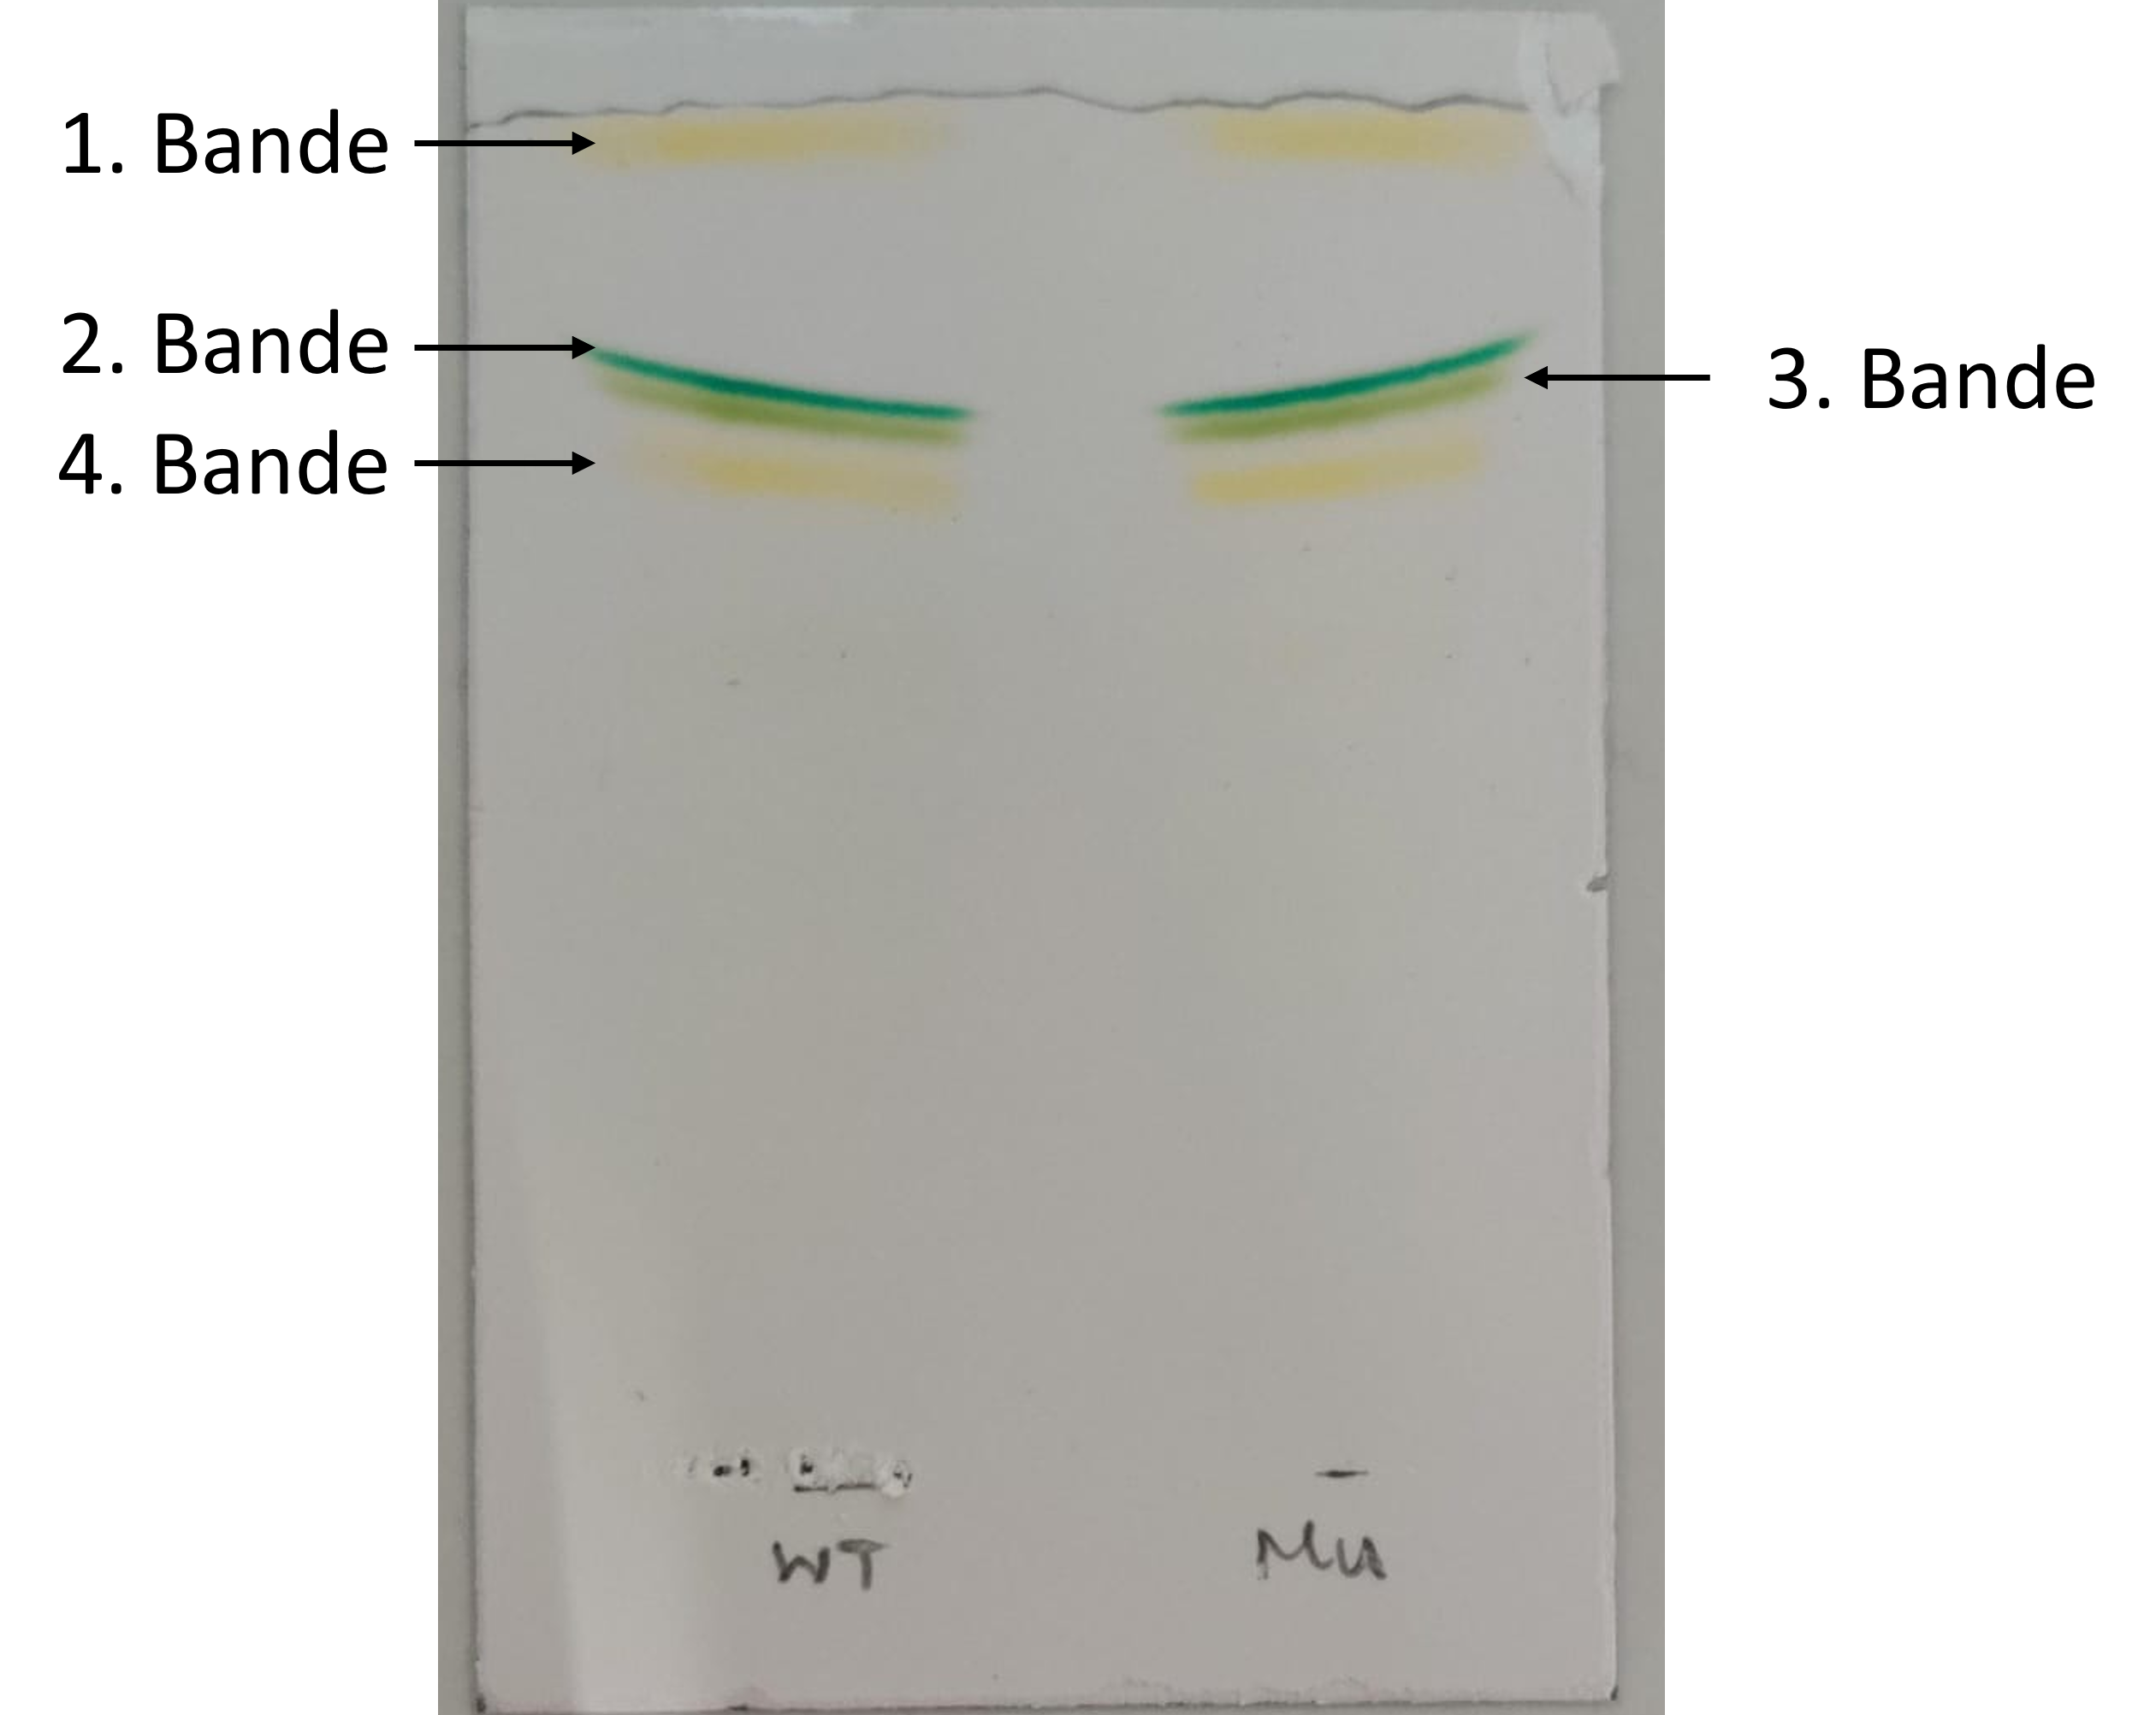
\includegraphics[scale=0.65]{DC-Plate_with_label.png}
				\caption{Probenauftrennung mittels Dünnschicht Chromatographie-Platte von der Spezies Nicotina tabacum (Wildtyp und FC1 - Mutant). Pigment wurden in Petrolether überführt und auf die Platte aufgetragen.}
				\label{fig:DC_Platte}
			\end{figure}
		
		Die Auftrennung der in Petrolether gelösten Pigmenten zeigen 4 stark gefärbte Banden (siehe Figure \ref{fig:DC_Platte}) bei beiden Nicotina tabacum Proben. Die jeweiligen Banden vom Wildtyp und Mutanten zeigen die gleichen $R_f$-Werte (siehe Tab \ref{tab:Rf_wert}) und auf der DC-Platte sind die vier Banden bei beiden Typen gleich schnell liefen.
		
			\begin{table}[H]
				\centering
				\caption{$R_f$-Werte von Band 1-4 aus Figure \ref{fig:DC_Platte} vom Nicotina Tabacum Wildtyp und Mutant.}
				\label{tab:Rf_wert}
				\begin{tabular}{ccc}
					\toprule
					Band&Wildtyp& Mutant\\
					\midrule
					1& 0.97 & 0.97\\
					2 & 0.79 & 0.79\\
					3 & 0.73 & 0.73 \\
					4 & 0.61 & 0.61\\
					\bottomrule
				\end{tabular}
			\end{table}	
			
			\begin{figure}[H]
				\centering
				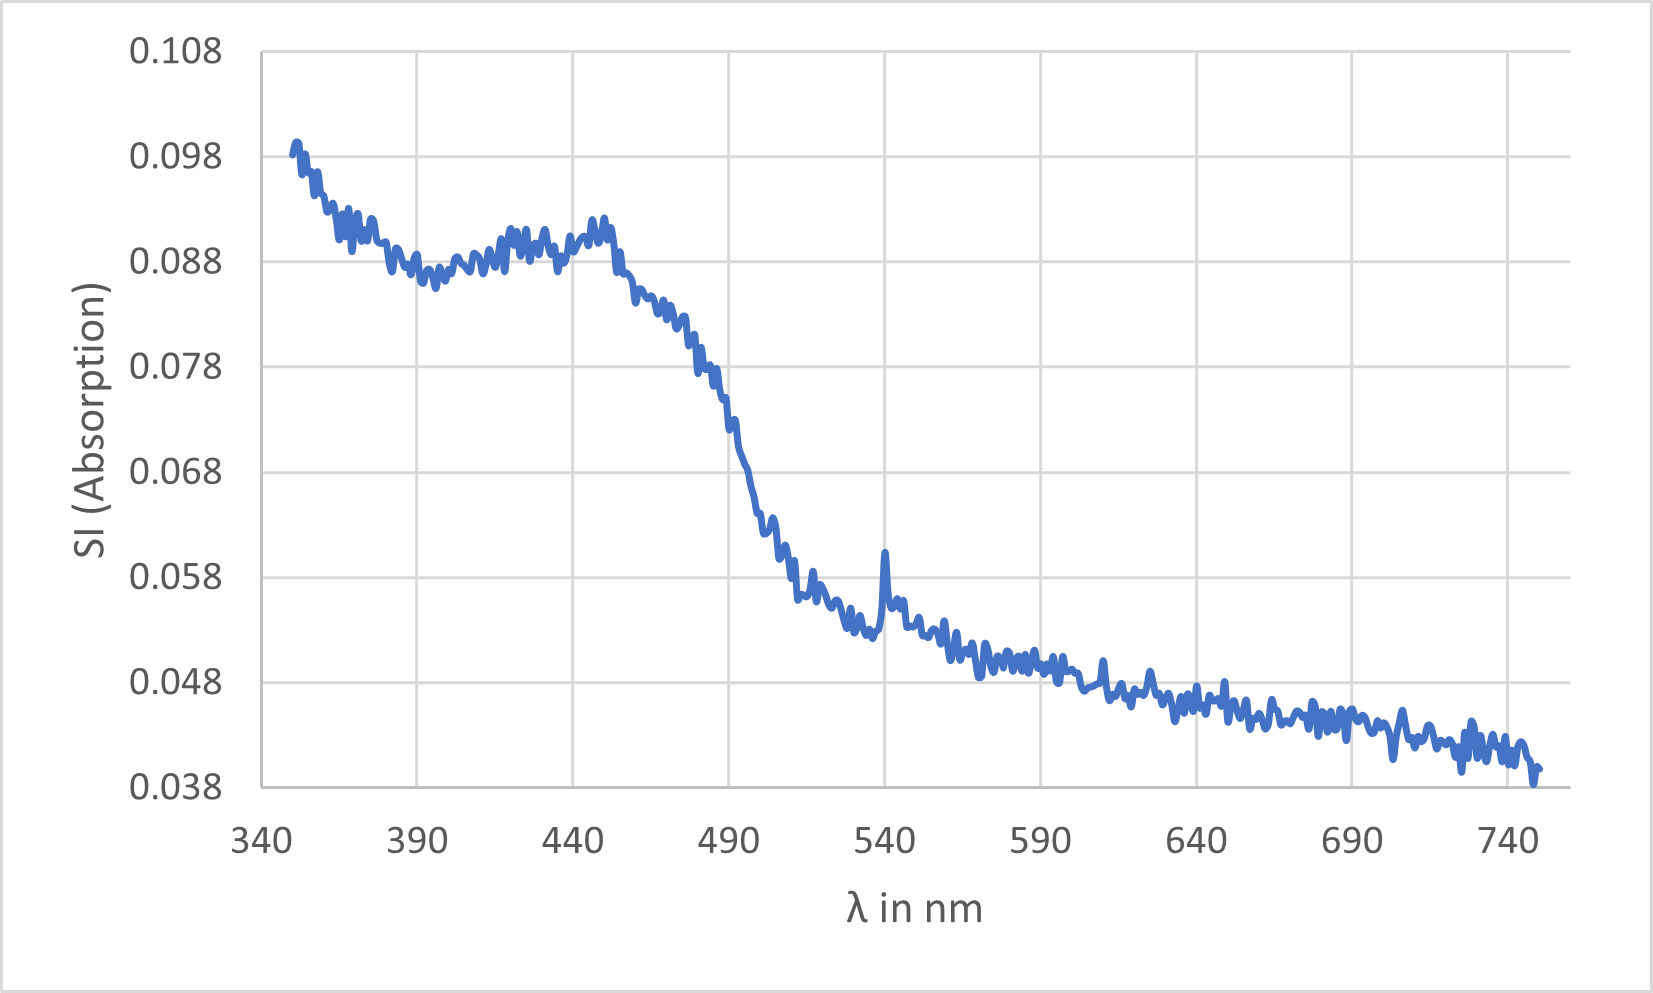
\includegraphics[scale=1]{firstband_axischange.png}
				\caption{Absoprtionsspektrum der ersten Bande aus Figure \ref{fig:DC_Platte}. Absorptionsmaxima liegt bei $\lambda$ = 400 bis 460 nm.}
				\label{fig:erste Bande}
			\end{figure}
			
			\begin{figure}[H]
				\centering
				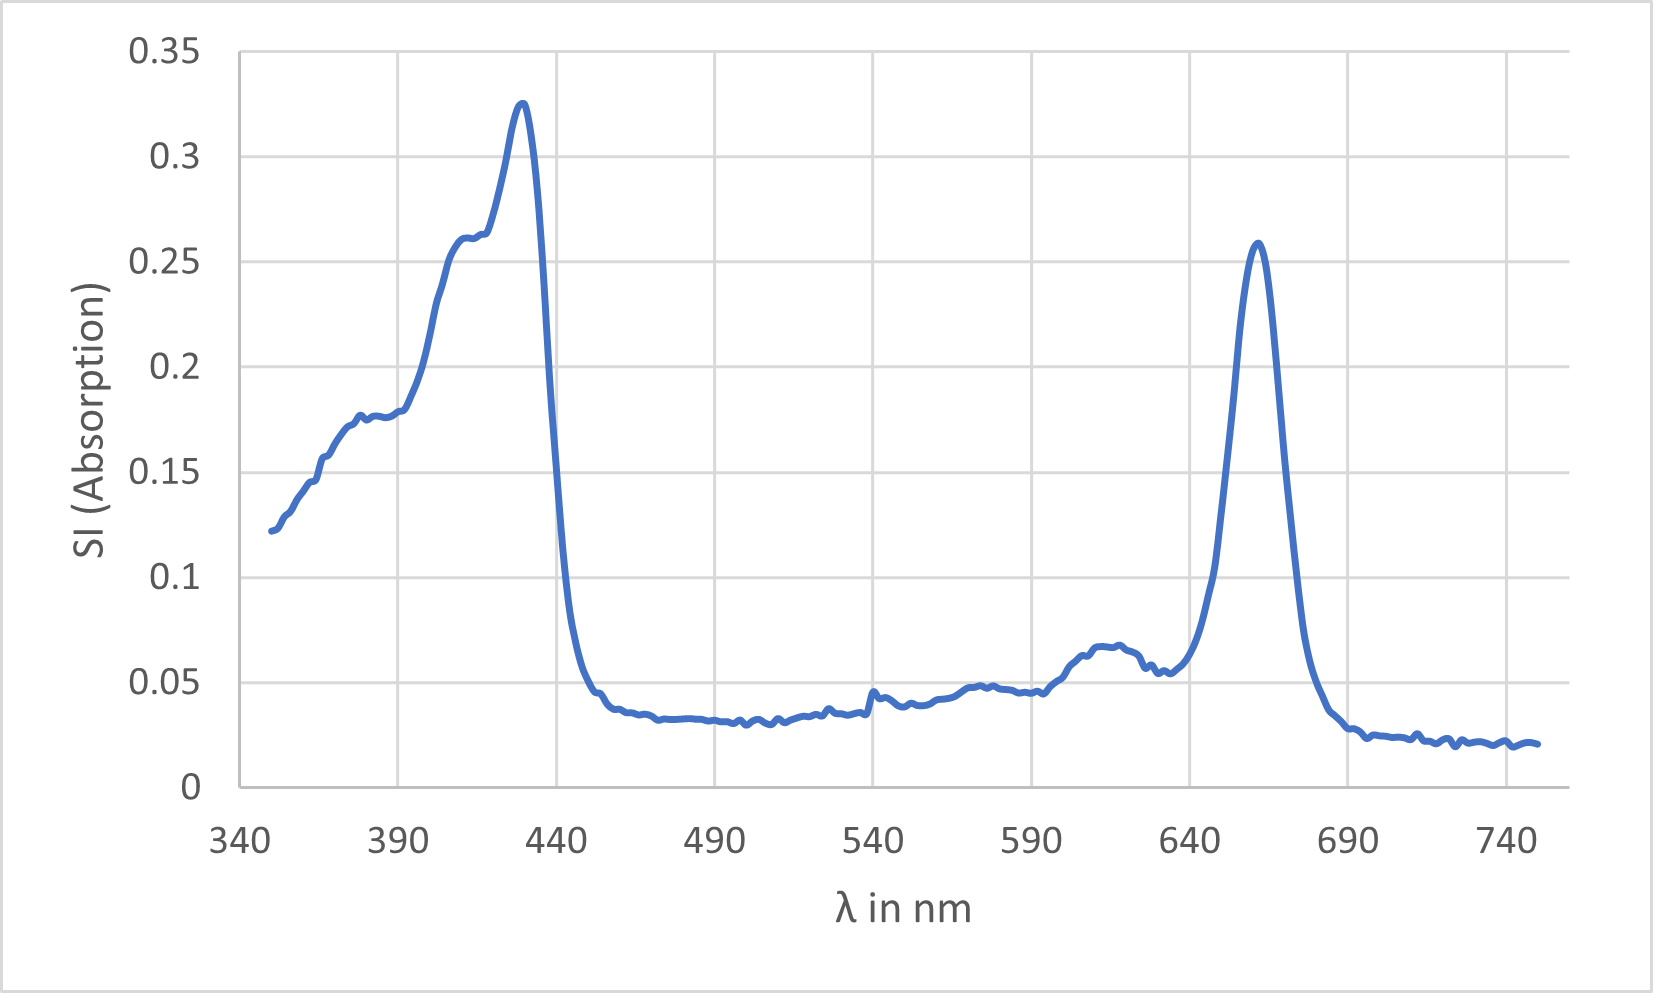
\includegraphics[scale=1]{secondband.png}
				\caption{Absoprtionsspektrum der zweiten Bande aus Figure \ref{fig:DC_Platte}. Absorptionsmaxima Bereich liegt im Bereich $\lambda$ = 430 und 664 nm.}
				\label{fig:zweite Bande}
			\end{figure}
			
			\begin{figure}[H]
				\centering
				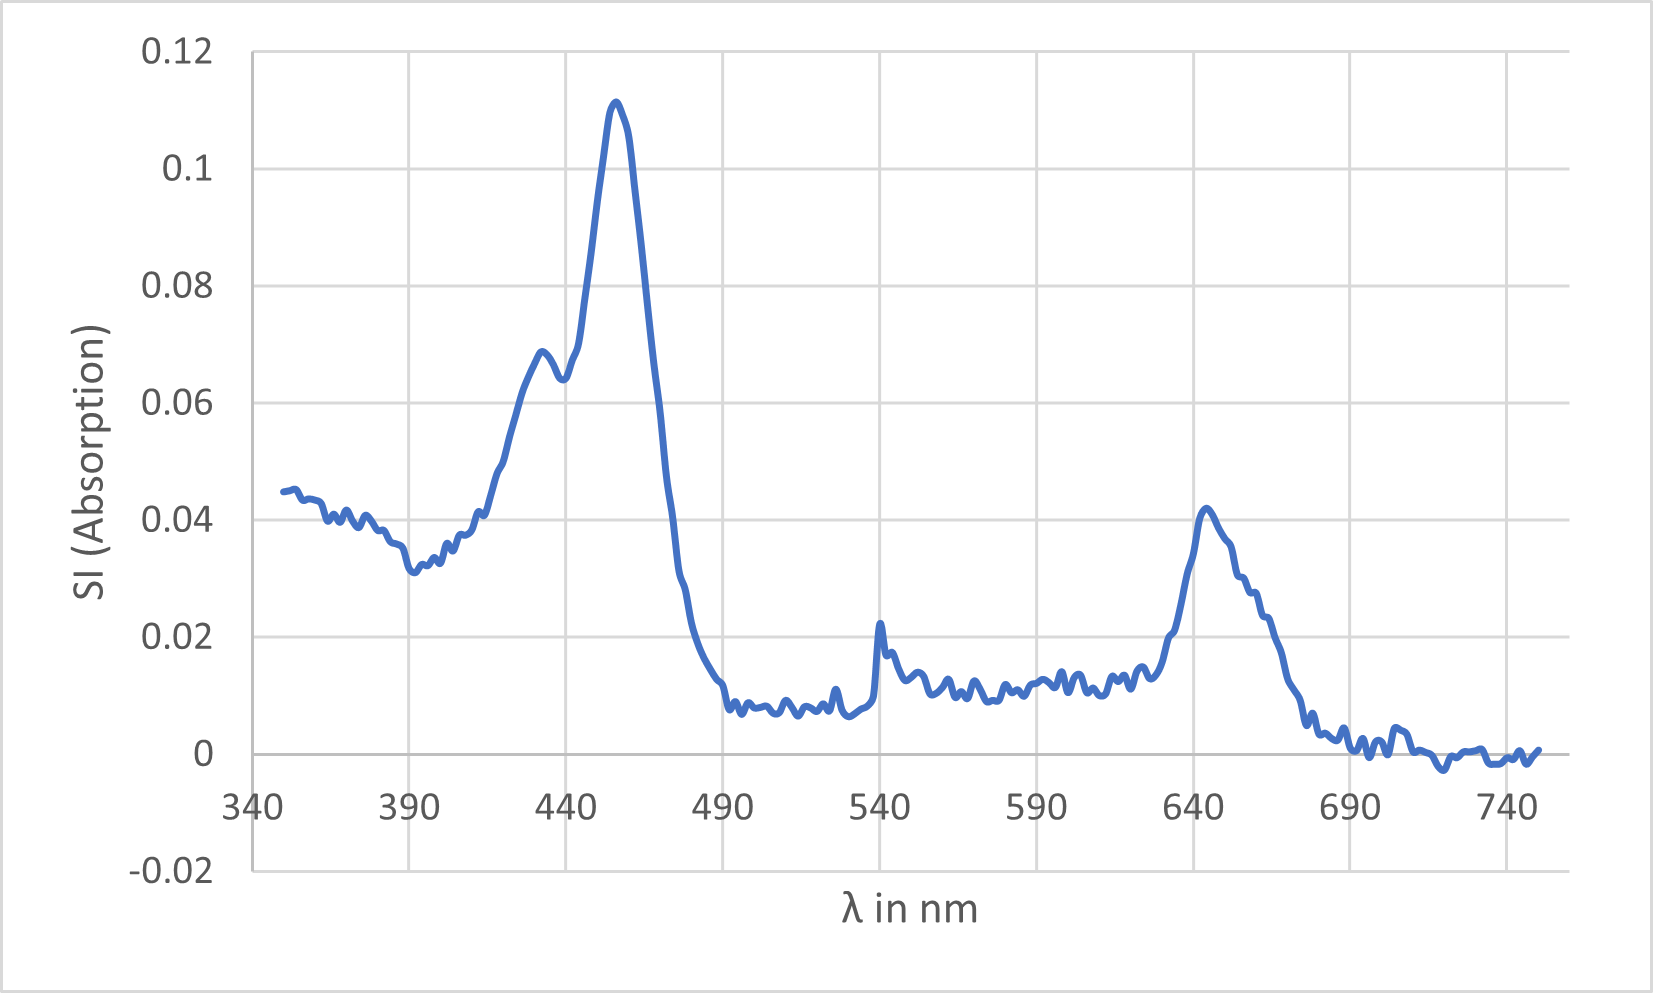
\includegraphics[scale=1]{thirdband.png}
				\caption{Absoprtionsspektrum der dritten Bande aus Figure \ref{fig:DC_Platte}. Absorptionsmaxima Bereich liegt im Bereich $\lambda$ = 458 und 646 nm. In diesen Absorption gibt es ein weiteren Peak bei $\lambda$ = 434 nm}
				\label{fig:dritte Bande}
			\end{figure}
			
			\begin{figure}[H]
				\centering
				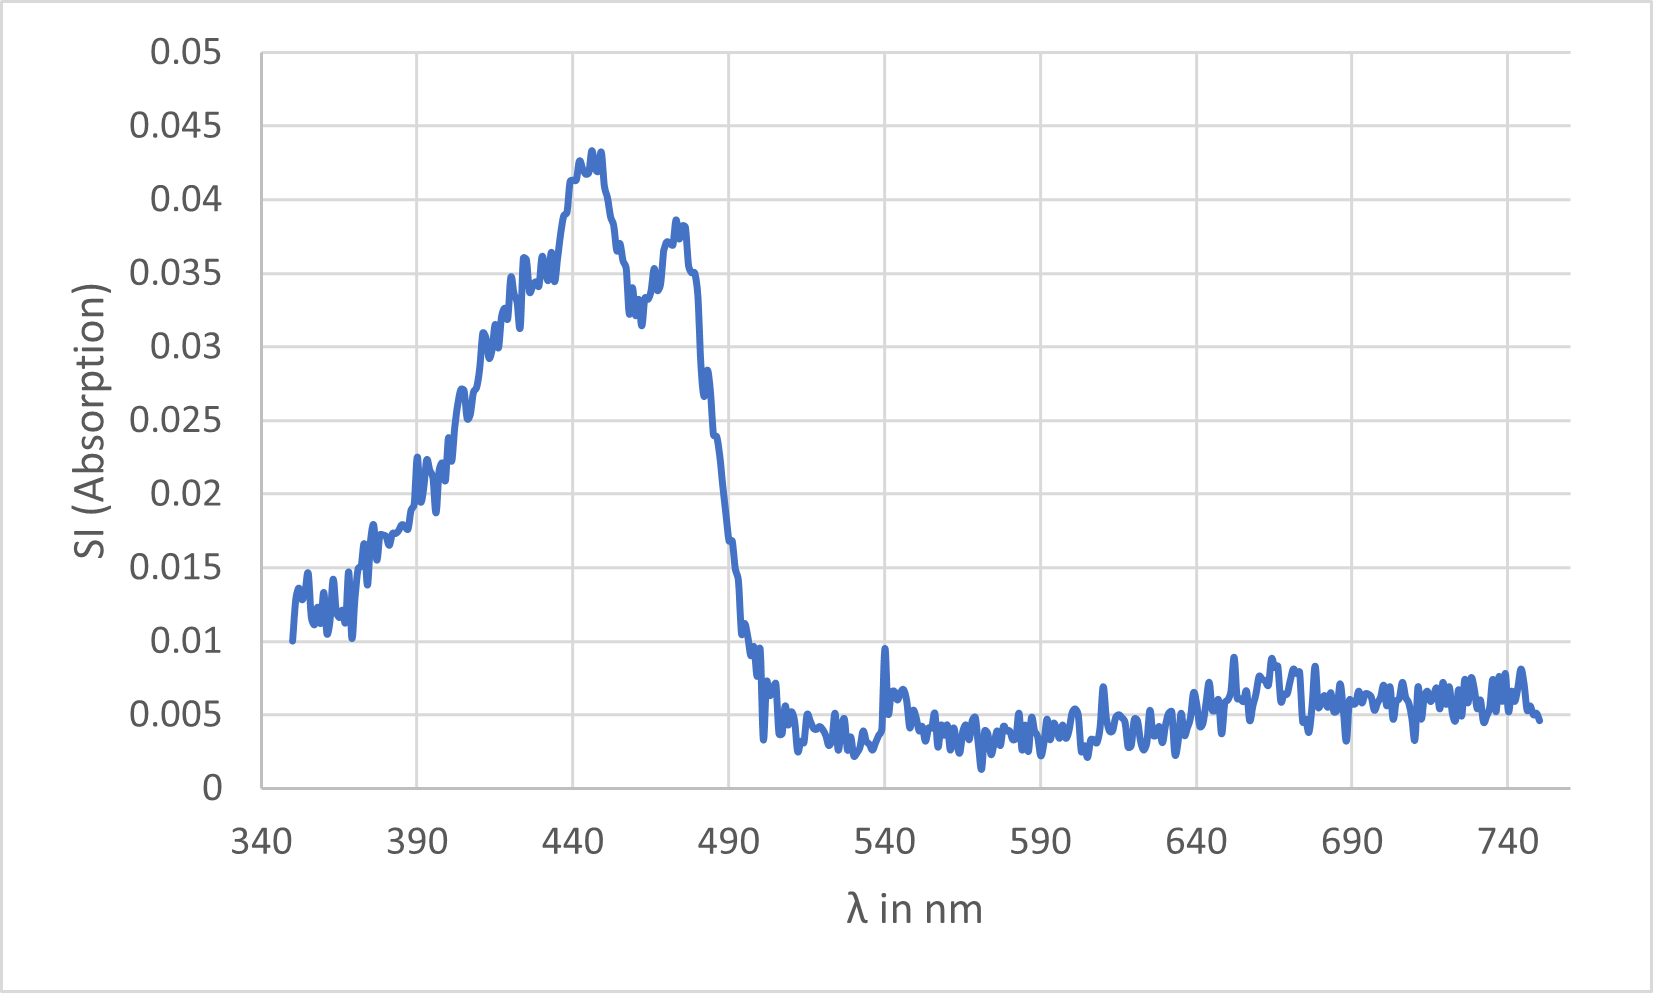
\includegraphics[scale=1]{fourthband.png}
				\caption{Absoprtionsspektrum der vierten Bande aus Figure \ref{fig:DC_Platte}. Absorptionsmaxima Bereich liegt im Bereich $\lambda$ = 448 und 476 nm.}
				\label{fig:vierte Bande}
			\end{figure}
			
			\begin{figure}[H]
				\centering
				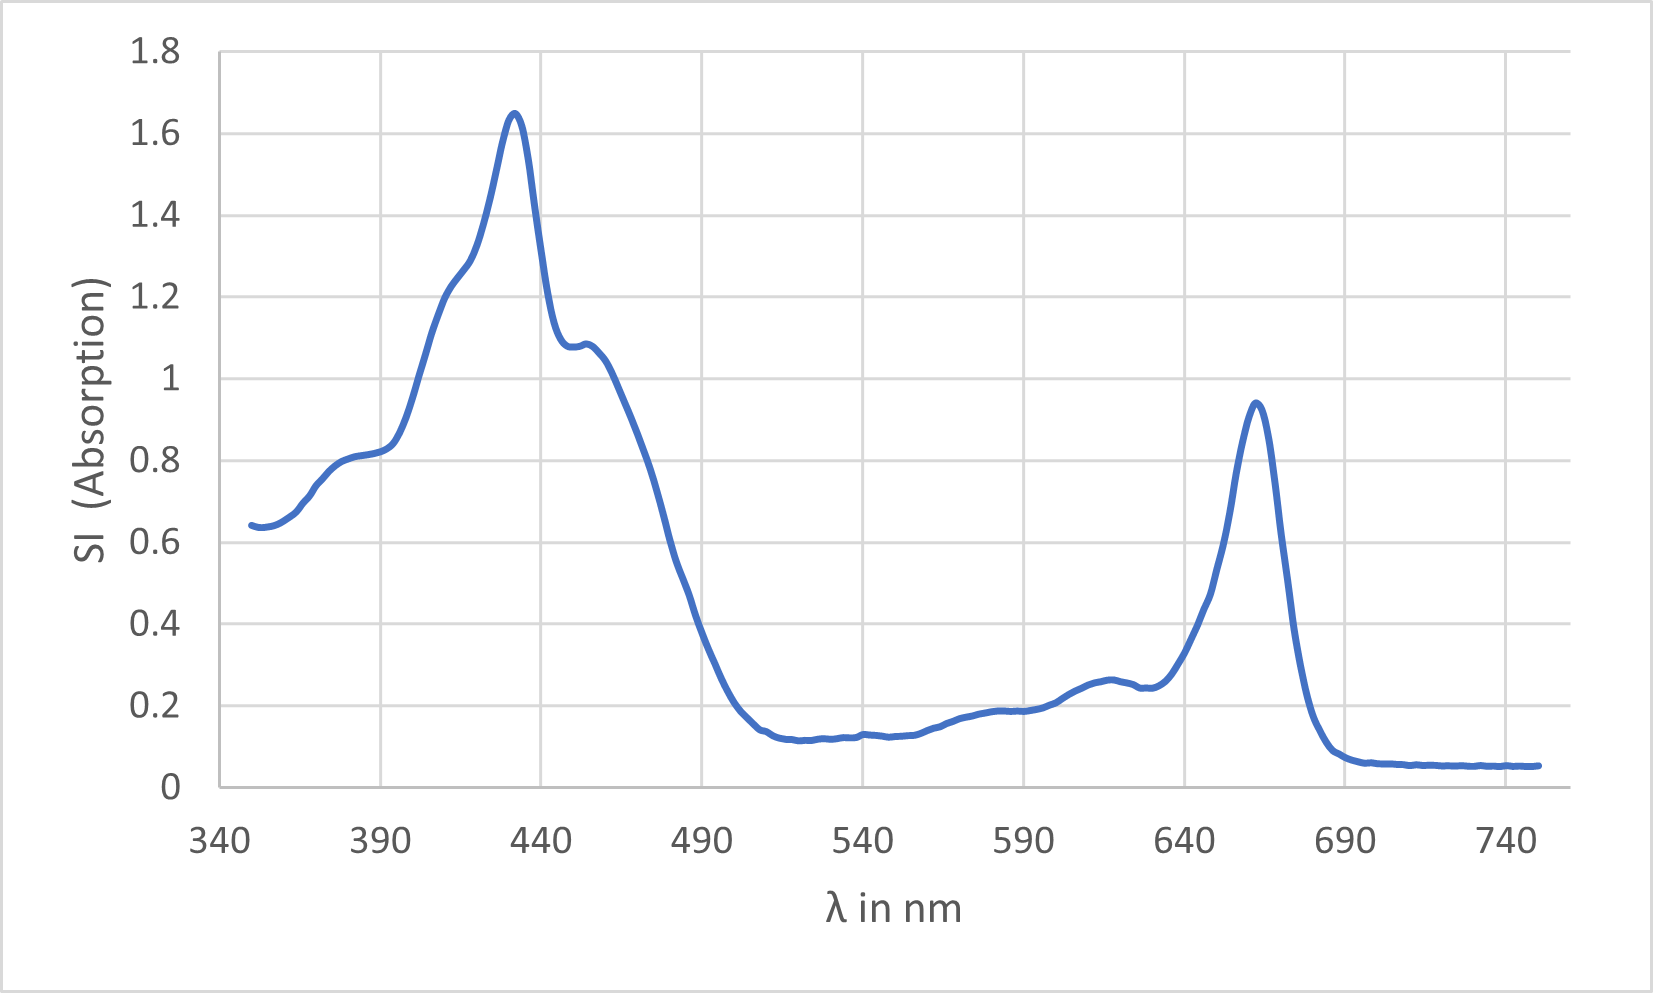
\includegraphics[scale=1]{fifthband.png}
				\caption{Absoprtionsspektrum vom unbekannten Pigmentextraktes.}
				\label{fig:fünfte Bande}
			\end{figure}
			
			Die Absorptionskurve der Bande 1 ist stark verrauschtzeigt ein Absorptionsmaximumbereich bei $\lambda$ = 400 - 460 nm (siehe Figure \ref{fig:erste Bande}).\\
			Bande 2 besitzt zwei Absorptionsmaxima bei $\lambda$ = 430 und 664 nm (siehe Figure \ref{fig:zweite Bande}). Zusätzlich sind noch zwei kleinen Peak bei  $\lambda$ = 412 nm und 614 nm in der Kurve zu sehen.\\
			In Figure \ref{fig:dritte Bande}  gibt es ebenfalls mehr als zwei Peaks. Zwei Absorptionsmaxima sind bei $\lambda$ = 458 und 646 nm und ein weiteren kleinen Peak bei $\lambda$ = 434 nm.\\
			Das Absorptionsspektrum von Bande 4 ist wie von Bande 1 etwas verrauscht und hat zwei Peaks bei $\lambda$ = 448 und 476 nm (siehe Figure \ref{fig:vierte Bande}).\\
			Bei den vier Absorptionsspektrum (Figure \ref{fig:erste Bande} - \ref{fig:vierte Bande}) existiert ein kleiner Peak bei $\lambda$ = 540 nm.\\
			Die vom Betreuer gegebene Pigmentextraktes zeigt mehrere Peaks (siehe Figure \ref{fig:fünfte Bande}), welches bei der Überlappung mit Bande zwei und drei Gemeinsamkeiten der Absorptionsmaxima zeigen (Siehe in Figure \ref{fig:kombinierteabsorptionsspektrum}). Ein Peak jedoch ist beim Pigmentxtrakt nicht zu sehen, welches bei Bande 3 zu sehen ist. Der Peak bei $\lambda$ = 646 nm wurde in Figure \ref{fig:kombinierteabsorptionsspektrum} rot hervorgehoben.\\
			Die Signalintensität des Pigmentextraktes ist circa 3 mal höher als die von Band 2 und 3.
			
			
			
			\begin{figure}[H]
				\centering
				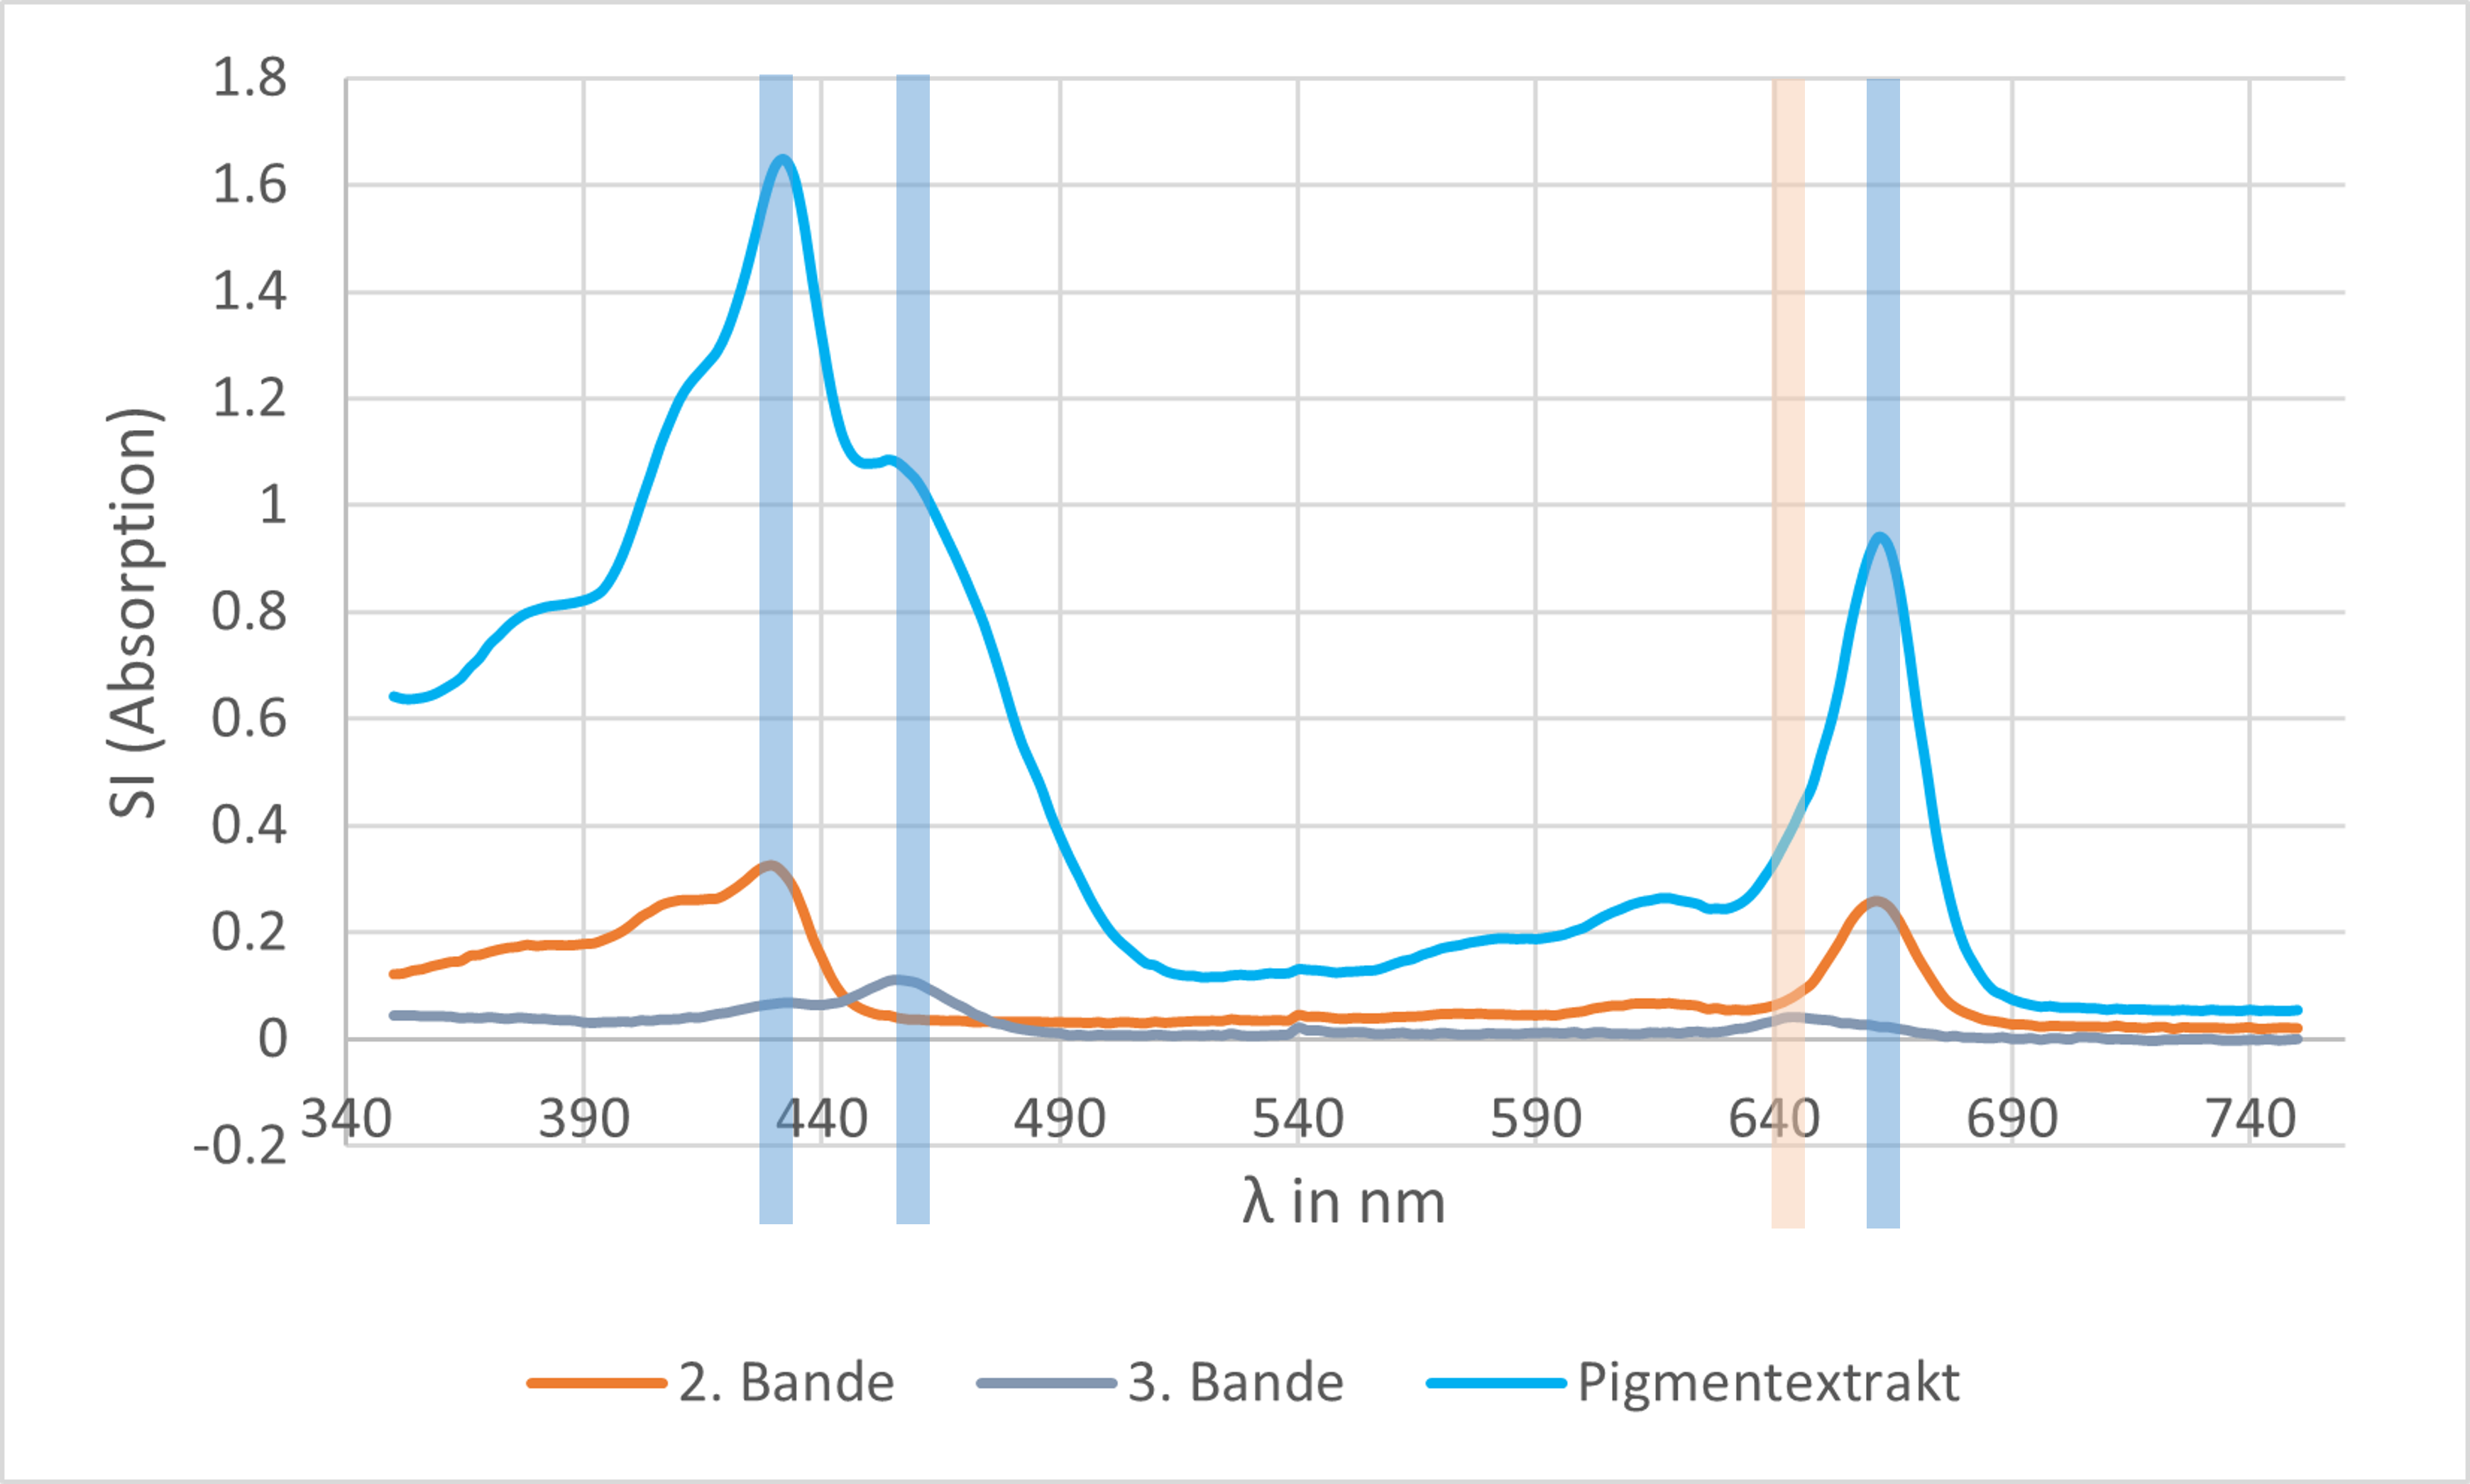
\includegraphics[scale=0.5]{combinedwithcommonpeaks_Pigmentextrakt.png}
				\caption{Vereintes Absorptionsspektrum von der unbekannten Probenextraktes, der zweiten und dritten Bande. Die Maximas der zweiten und dritten Bande wurde hier farblich hervorgehoben. Die rote Markierung zeigt ein fehlenden Peak bei der unbekannte Probeextraktes}
				\label{fig:kombinierteabsorptionsspektrum}
			\end{figure}
			
			
				
	\section{Diskussion}
	Aus der Nicotina Tabacum Pflanze wurde von der FC1-Antisense Mutante mehr Chlorophylle a und b als beim Wildtyp extrahiert(siehe Table \ref{tab:konzentration chl a und b}).\\
	Da beide Proben mit der gleichen Mengen an Volumina bei der DC-Auftrennung weitergearbeitet wurde, ist auch bei den Banden zwischen den beiden Typen kein Farbintensitätsunterschied zu erkennen (Figure \ref{fig:DC_Platte}).\\

	Die Identifikation der 4 Banden bei der DC-Platte wurde ein Absoptionsspektrum aufgenommen und mit den Literaturwerten von Heather A. Hager \cite{Absorption_Maxima_Carotinoide} und Peter von Sengbusch\cite{Absorption_Maxima_Chlorophylle} verglichen.
	
	
	
	
	\section{Anhang}
		\subsection{Rechenwege}
			\begin{figure}[H]
				\centering
				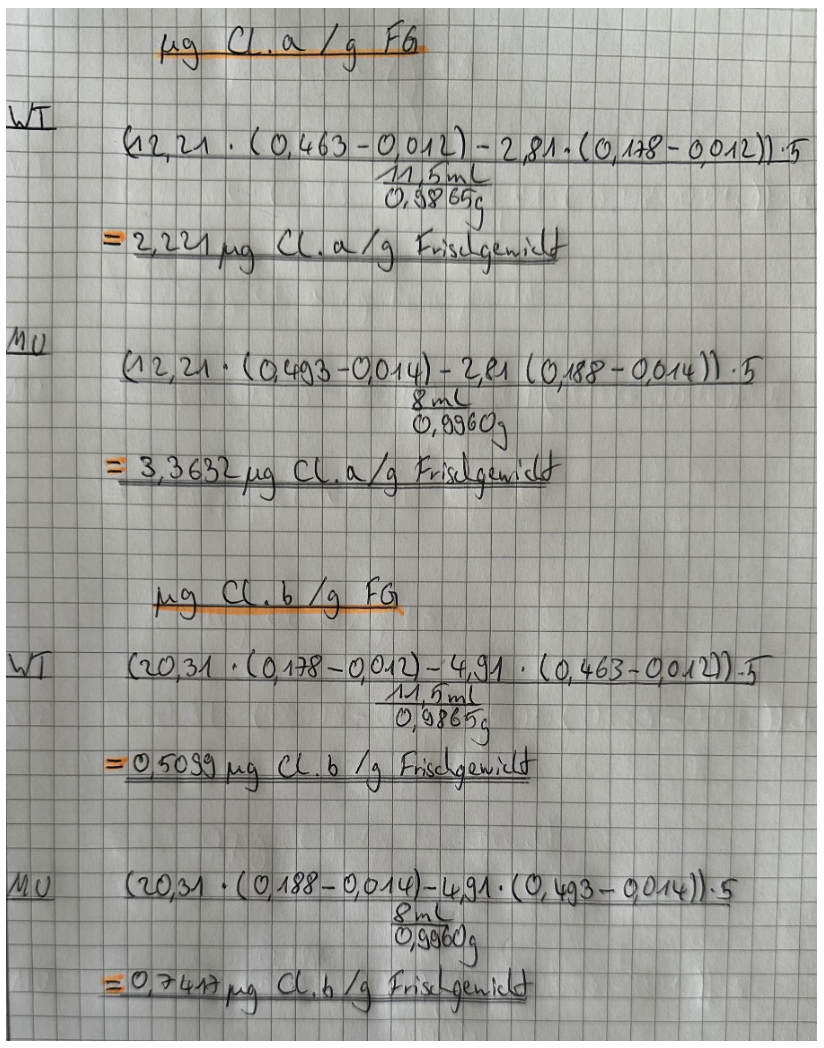
\includegraphics[scale=0.8]{Rechenweg_frido}
				\caption{Rechenweg der Konzentrationsbestimmung von Chlorophylle a und b des Rohextraktes. Absorptionswerte bei den jeweiligen Wellenlänge $\lambda$ = 470, 646, 663 und 720 nm wurde aus der Table \ref{tab:Rohdaten Extinktion Rohextraktes} entnommen.}
				\label{fig:Konzentrationsbestimmungrechenweg}
			\end{figure}
		\subsection{Rohdaten}
			\subsubsection{Einwaage der Proben }
				\begin{table}[H]
					\centering
					\caption{Masse der Blätter und das Volumen des in basischen Aceton extrahierten Pigmenten vom Nicotiana tobacum des Wildtyps und FC1-Antisense Mutant}
					\label{tab:Probemassen und Volumen}
					\begin{tabular}{ccc}
						\toprule
						&Wildtyp& Mutant\\
						\midrule
						m(Frischgewicht) in g & 0.9965 & 0.9960\\
						V(Rohextrakt) in mL & 11.5 & 8\\
						\bottomrule
					\end{tabular}
				\end{table}
				
			\subsubsection{Extinktion des Rohextraktes}
				\begin{table}[H]
					\centering
					\caption{Die Extinktion des Rohextraktes vom Wildtyp und Mutant in basischen Aceton wurde bei $\lambda$ = 470, 646, 663, 720 nm gemessen. Als Blank wurde die Extraktionslösung (100$\%$ Aceton und 20 mM NH$_4$OH) verwendet.
					Die Proben wurden jeweils 1:5 mit der Extraktionslösung verdünnt.}
					\label{tab:Rohdaten Extinktion Rohextraktes}
					\begin{tabular}{ccccc}
						\toprule
						$\lambda$ in nm &470& 646 & 663 & 720\\
						\midrule
						Wildtyp &0.424 & 0.178 & 0.463 & 0.012\\
						Mutant & 0.423 & 0.188 & 0.493 & 0.014 \\
						\bottomrule
					\end{tabular}
				\end{table}
			
			\subsubsection{Substanzstrecke auf der DC-Platte}
				\begin{table}[H]
					\centering
					\caption{Substanzstrecke der 4 Banden aus Figure \ref{fig:DC_Platte} für den Wildtyp (WT) und der FC1-Mutante (MU). Die Laufmittelfront-Distanz beträgt 6.2 cm}
					\label{tab:Distance_Rf_Werte_Banden_Rohwerte}
					\begin{tabular}{cc}
						\toprule
						Substanzstrecke Wildtyp in cm& Substanzstrecke Mutant in cm\\
						\midrule
						6.0 & 6.0 \\
						4.9 & 4.9\\
						4.5 & 4.5\\
						3.8 & 3.8\\
						\bottomrule
					\end{tabular}
				\end{table}


	\bibliographystyle{plainurl}
	\nocite{*}
	\bibliography{Literatur}
	\newpage
	
\end{document}